\documentclass[a4paper]{article} 
\input{latex/head}
\begin{document}

%-------------------------------
%	TITLE SECTION
%-------------------------------

\fancyhead[C]{}
\hrule \medskip % Upper rule
\begin{minipage}{0.295\textwidth} 
\raggedright
\footnotesize
Dylan Huber 
\end{minipage}
\begin{minipage}{0.4\textwidth} 
\centering 
\large 
Pipette Lab Write-up\\ 
\normalsize 
02-261\\ 
\end{minipage}
\begin{minipage}{0.295\textwidth} 
\raggedleft
\today\hfill\\
\end{minipage}
\medskip\hrule 
\bigskip

%-------------------------------
%	CONTENTS
%-------------------------------

\section{Results and Figures}
\subsection{Tool Comparison}

\begin{figure}[H]
    \centering
    \includegraphics[width=1\linewidth]{tool.png}
    \caption{This experiment was performed on water. The pipette man has higher accuracy and 
    precision compared to the pipette aid. Both tools undershoot fairly consistently.}
\end{figure}

From this figure we can conclude that the pipette man is more precise and accurate. However, the
pipette man seems to be poorly calibrated throughout this entire lab. Despite having it at exactly
.500 ml, the pipette always undershot by $.010 - .015$ml. The error for the pipette aid is due to
a combination of the limits of the tool and the skill or lack thereof of the user.

\subsection{Liquid Comparison}

\begin{figure}[H]
    \centering
    \includegraphics[width=1\linewidth]{liquid.png}
    \caption{This experiment was performed was performed with the pipette man. Results have been
    normalized to their target weight, which was .5g for the water, and .526g for the 20\% 
    glycerol. We can see that the water had higher precision and higher accuracy.}
\end{figure}

From this we can conclude that the pipette man works much better with water. It has higher accuracy
and precision compared to using the 20\% glycerol solution. During the lab we noticed that it was
difficult to get the entirety of the glycerol solution out of the pipette man, which is probably
the reason for the severe undershooting.

\subsection{Volume Comparison}

\begin{figure}[H]
    \centering
    \includegraphics[width=.7\linewidth]{vol.png}
    \caption{This experiment was performed on water using the pipette man. Results have been
    normalized to the proportion of the target. The .5ml target is more accurate and precise than
    the .2ml target.}
\end{figure}



From this figure we can conclude that using the pipette man on volumes higher in the range of the
tool helps increase proportional percision and accuracy. From the figure below, we can see that 
in real values, the .2ml target seems to have better accuracy, but still worse precision. Perhaps
shows that the underhsooting issue we see throughout this lab scales with volume. 

\begin{figure}[H]
    \centering
    \includegraphics[width=.7\linewidth]{vol2.png}
    \caption{Same as figure 3, but with real difference from target in ml.}
\end{figure}

\subsection{People Comparison}

\begin{figure}[H]
    \centering
    \includegraphics[width=1\linewidth]{people.png}
    \caption{This experiment was performed on water with the pipette aid and a .5ml target. Dylan
    has the best accuracy and precision (except one outlier). Luke seems to have the second best
    while Joseph should work on his pipetting.}
\end{figure}

From this we can conclude that I am the best at pipetting within our group and Joseph is the worst.
This means that I should be in charge of pipetting for future labs.

\newpage

%------------------------------------------------

\section{Experimental Issues}

\subsection{Human Error}

Even in the sections which were not intented to measure the skill of our scientists, their skill
was tested. A more skilled pipetter might have had significantly better results with both the
pipette man and the pipette aid.

\subsection{Material Error}

As mentioned before, the pipette man significantly undershot for the entirety of the lab. Perhaps
this issue could have been fixed via tuning the pipette man in some way or replacing it with a
different one. 

\subsection{Evaporation}

In the weigh boat, our liquid spread out significantly. This gave it large surface area making
evaportation non-negligable. This caused the measurements to rapidly decrease while we were 
reading them, perhaps adding to the undershooting.

\subsection{Splashing}

Sometimes when depositing liquid into the weigh boat, it would splash onto the rear wall of the
scale. This was especially prevalent when Joseph was pipetting. This would also cause a decrease
in the read weight.

\bigskip

\section{Data Table:}

\begin{figure}[H]
    \centering
    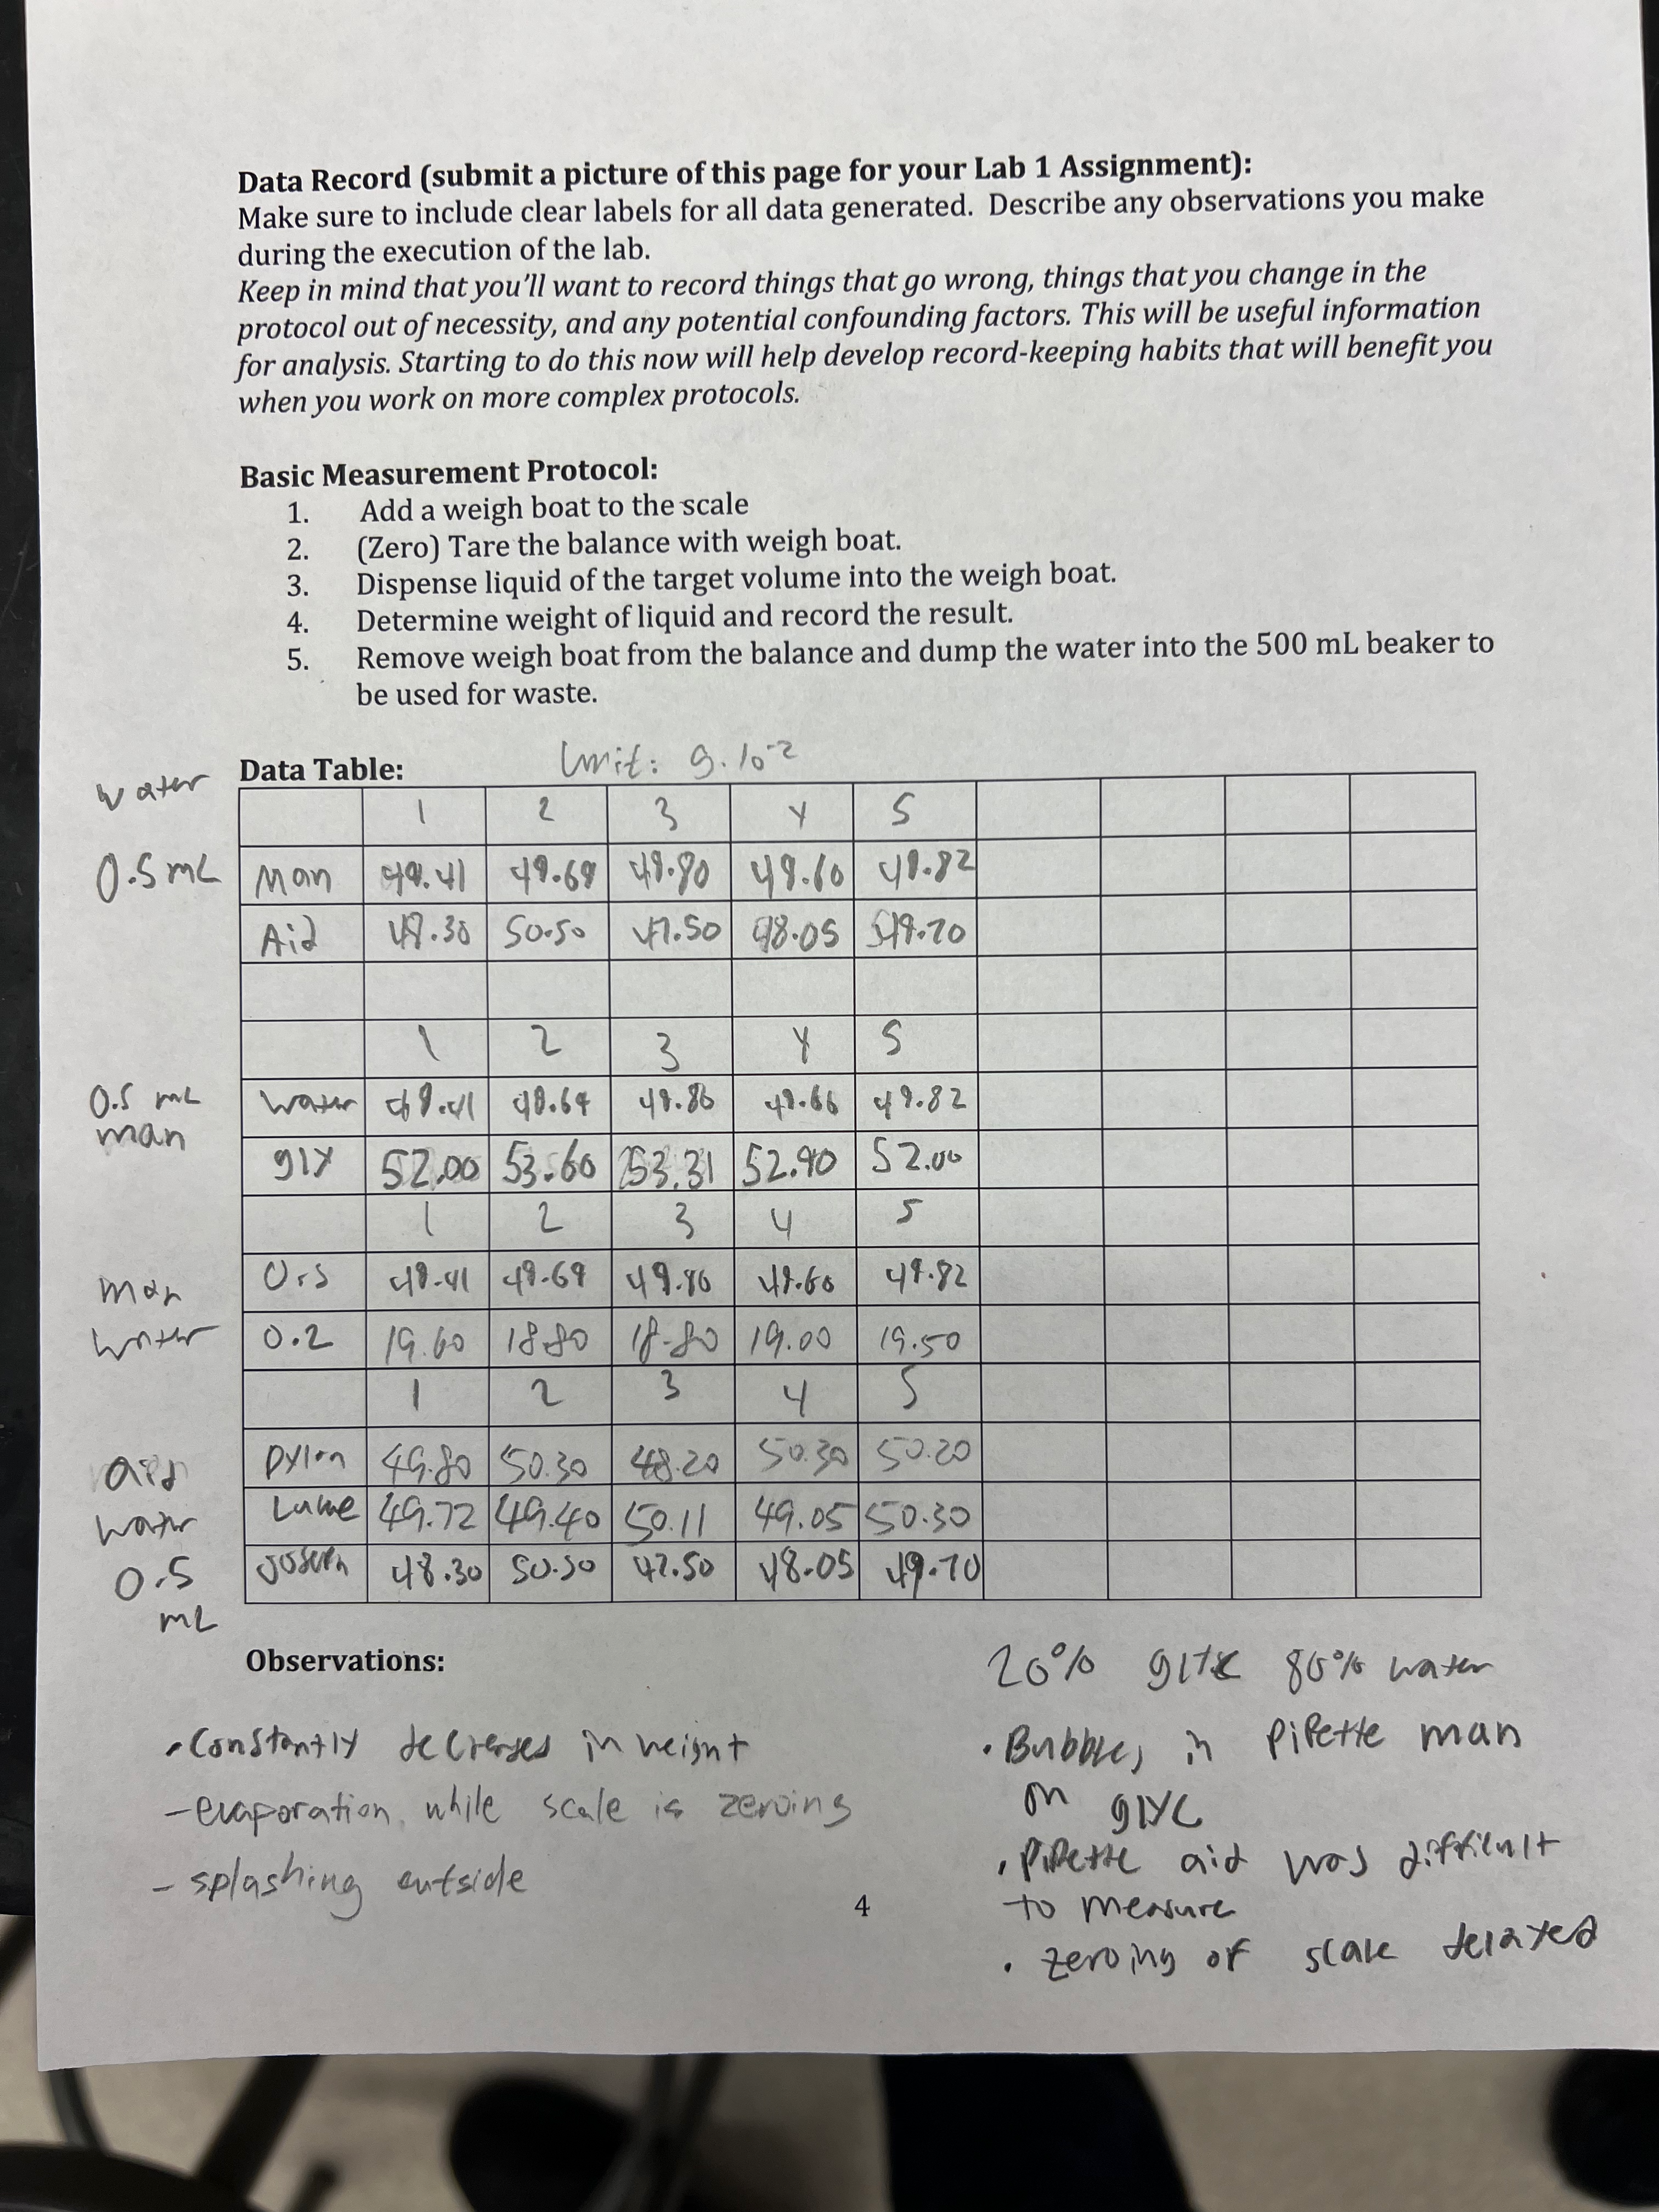
\includegraphics[width=1\linewidth]{IMG_8965.png}
\end{figure}

%------------------------------------------------

\end{document}